\documentclass{standalone}
\usepackage{tikz}
\begin{document}
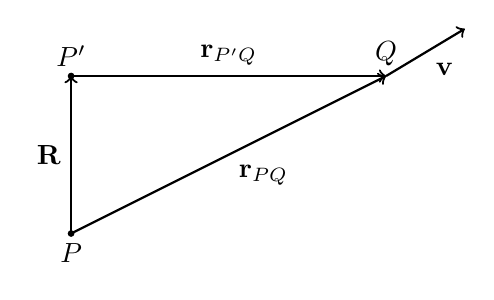
\begin{tikzpicture}[scale=2]
    \filldraw[black](0,0)node[above]{$P'$}circle(0.5pt);
    \filldraw[black](0,-1)node[below]{$P$}circle(0.5pt);
    \draw[->,thick](0,-1)--(0,0)node[midway, left]{$\mathbf{R}$};


    \filldraw[black](2,0)node[above]{$Q$};
    \draw[->,thick](2,0)--(2.5,0.3)node[midway, below right]{$\mathbf{v}$};

    \draw[->,thick](0,0)--(2,0)node[midway, above]{$\mathbf{r}_{P'Q}$};
    \draw[->,thick](0,-1)--(2,0)node[midway, below right]{$\mathbf{r}_{PQ}$};
\end{tikzpicture}
\end{document}